\documentclass[11pt]{article}
\usepackage[utf8]{inputenc}	% Para caracteres en español
\usepackage{amsmath,amsthm,amsfonts,amssymb,amscd}
\usepackage{multirow,booktabs}
\usepackage[table]{xcolor}
\usepackage{fullpage}
\usepackage{lastpage}
\usepackage{enumitem}
\usepackage{fancyhdr}
\usepackage{mathrsfs}
\usepackage{wrapfig}
\usepackage{setspace}
\usepackage{calc}
\usepackage{multicol}
\usepackage{cancel}
\usepackage[retainorgcmds]{IEEEtrantools}
\usepackage[margin=1cm]{geometry}
\usepackage{amsmath}
\newlength{\tabcont}
\setlength{\parindent}{0.0in}
\setlength{\parskip}{0.05in}
\usepackage{empheq}
\usepackage{framed}
\usepackage[most]{tcolorbox}
\usepackage{xcolor}
\usepackage{graphicx}
\usepackage{listings}
% -- Basic formatting
\usepackage[utf8]{inputenc}
\usepackage[english]{babel}
\usepackage{times}
\usepackage{caption}
\usepackage{subcaption}
\usepackage{placeins}
\setlength{\parindent}{0pt}
\usepackage{indentfirst}% -- Defining colors:
\usepackage[dvipsnames]{xcolor}
\definecolor{codegreen}{rgb}{0,0.6,0}
\definecolor{codegray}{rgb}{0.5,0.5,0.5}
\definecolor{codepurple}{rgb}{0.58,0,0.82}
\definecolor{backcolour}{rgb}{0.95,0.95,0.92}% Definig a custom style:
\lstdefinestyle{mystyle}{
    backgroundcolor=\color{backcolour},   
    commentstyle=\color{codepurple},
    keywordstyle=\color{NavyBlue},
    numberstyle=\tiny\color{codegray},
    stringstyle=\color{codepurple},
    basicstyle=\ttfamily\footnotesize\bfseries,
    breakatwhitespace=false,         
    breaklines=true,                 
    captionpos=t,                    
    keepspaces=true,                 
    numbers=left,                    
    numbersep=5pt,                  
    showspaces=false,                
    showstringspaces=false,
    showtabs=false,                  
    tabsize=2
}% -- Setting up the custom style:
\lstset{style=mystyle}
\lstset{
  style=mystyle,
  framexleftmargin=3.5mm,
  rulesepcolor=\color{black},
  linewidth=0.6\linewidth,
  xleftmargin=12pt,
  aboveskip=12pt,
  belowskip=12pt
}
\colorlet{shadecolor}{orange!15}
\parindent 0in
\parskip 1pt
\geometry{margin=1in, headsep=0.25in}
\theoremstyle{definition}
\newtheorem{defn}{Definition}
\newtheorem{reg}{Rule}
\newtheorem{exer}{Exercise}
\newtheorem{note}{Note}
\graphicspath{ {./images/} }
\linespread{0.75}
\begin{document}
\setcounter{section}{0}
\title{MIE223 Lecture Notes}

\thispagestyle{empty}

\begin{center}
{\LARGE \bf Foundations of Knowledge Graphs}\\
{\large MIE223}\\
Winter 2025
\end{center}
\section{Knowledge Graphs}

\subsection{Knowledge Graphs}
Knowledge
Graphs

\begin{itemize}
    \item “Triple” data on web
    \item Distributed, dynamic
    \begin{itemize}
        \item Some controlled sources: WikiData
    \end{itemize}
    \item Nodes are entities
    \item Edges are labeled by relations (linked data)
    \item Foundation in RDF
\end{itemize}

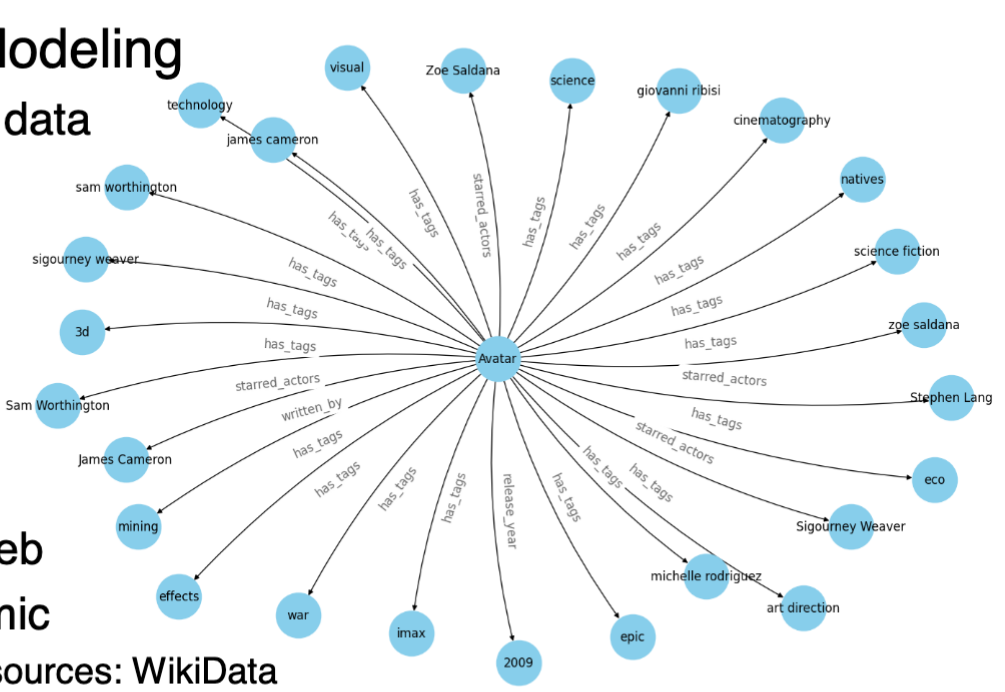
\includegraphics[width=\textwidth/2]{1.png}

\subsection{The Resource Description Framework Is
All About Making Statements}

\begin{itemize}
    \item A statement can be thought of as an ordered triple composed of three items:
    (resource, predicate, value)
    \item A Resource is anything that can be identified.
    \item A Predicate is a property name that has a URI. The Predicate may or may not
    actually be resolvable.
    \item A Value is another Resource or a literal.
    \item Statements may be represented in RDF XML, abbreviated RDF XML,
    or (locally) graphs
    \item We want to state world knowledge in a structured format
\end{itemize}

Why?

\begin{itemize}
    \item A Dynamic Source of Structured Data
    \begin{itemize}
        \item Query it dynamically on the web from different sources (SPARQL)
        \item Inherently linked (entities and relations are shared) across sources
        \begin{itemize}
            \item See schema.org
        \end{itemize}
    \end{itemize}
    \item Question Answering
    \begin{itemize}
        \item When was William G. Davis born?
        \item Who was the first woman in space? What year?
    \end{itemize}
    \item Entity Resolution
    \begin{itemize}
        \item You search for Michael Jordan
        \item The basketball player, the professor, the general?
        \item Important for search
    \end{itemize}
\end{itemize}

\section{Entity Resolution}
\subsection{Common task: Information Retrieval (i.e., Google)}

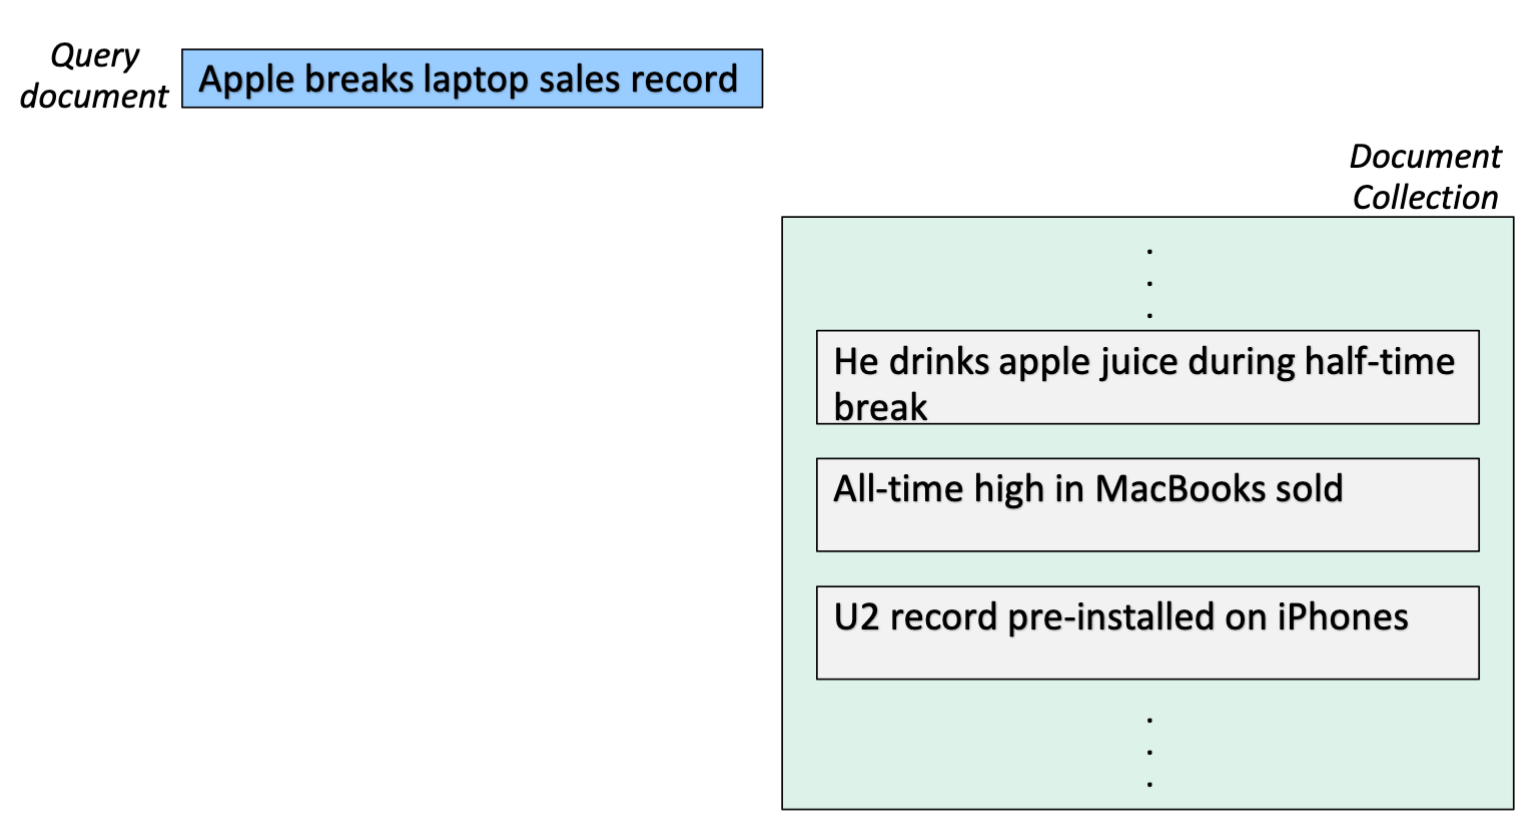
\includegraphics[width=\textwidth/2-2.08049pt]{2.png}
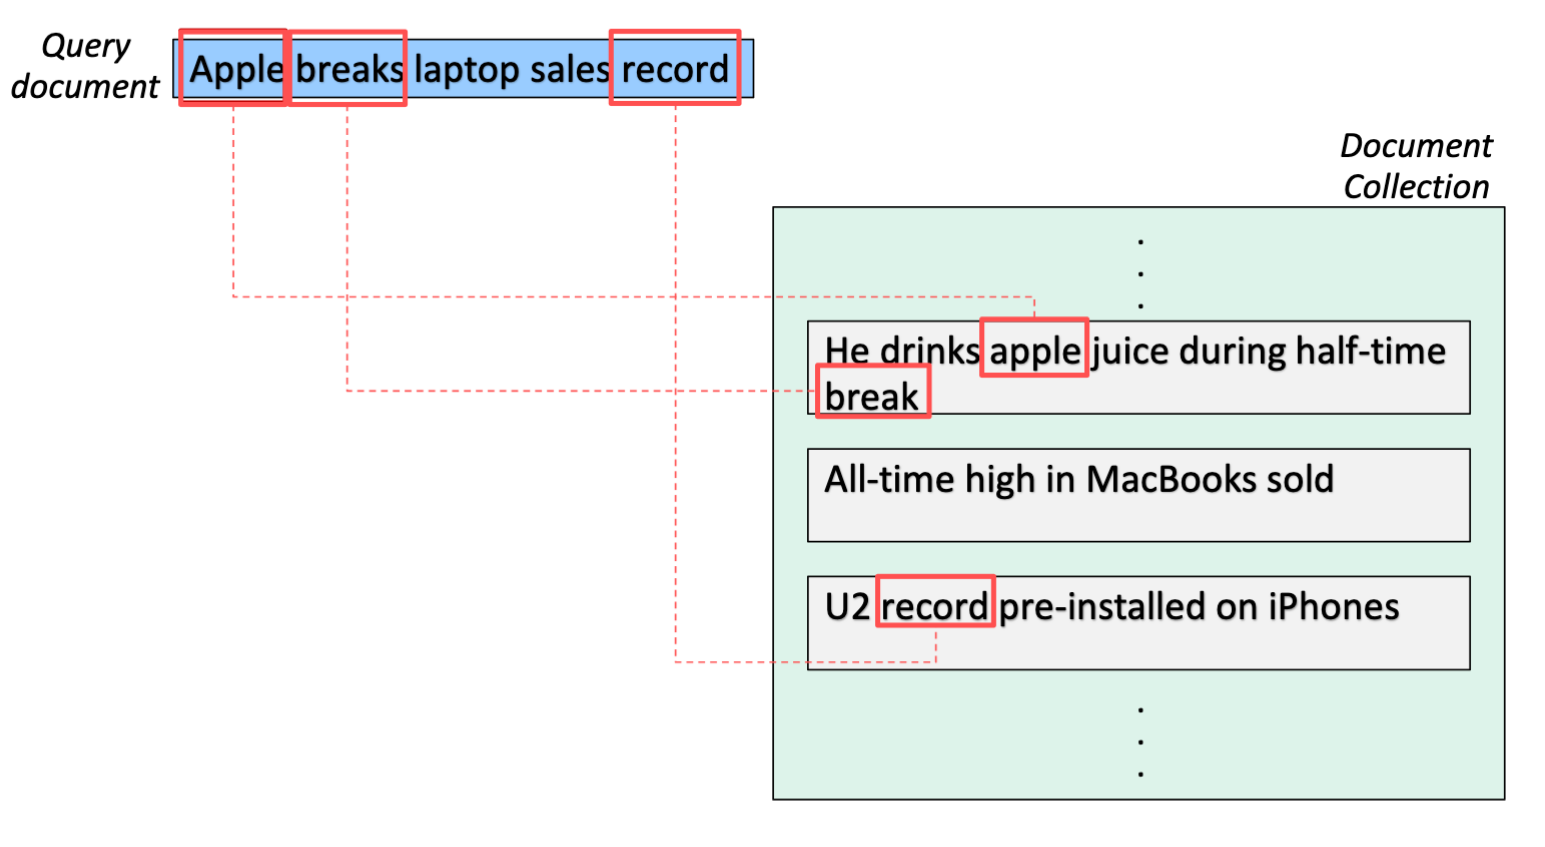
\includegraphics[width=\textwidth/2]{3.png}

Matching words do not always indicate similarity.
the query does not match the ideal article


Word co-occurrence can be misleading, too.
apple still matches apple juice.

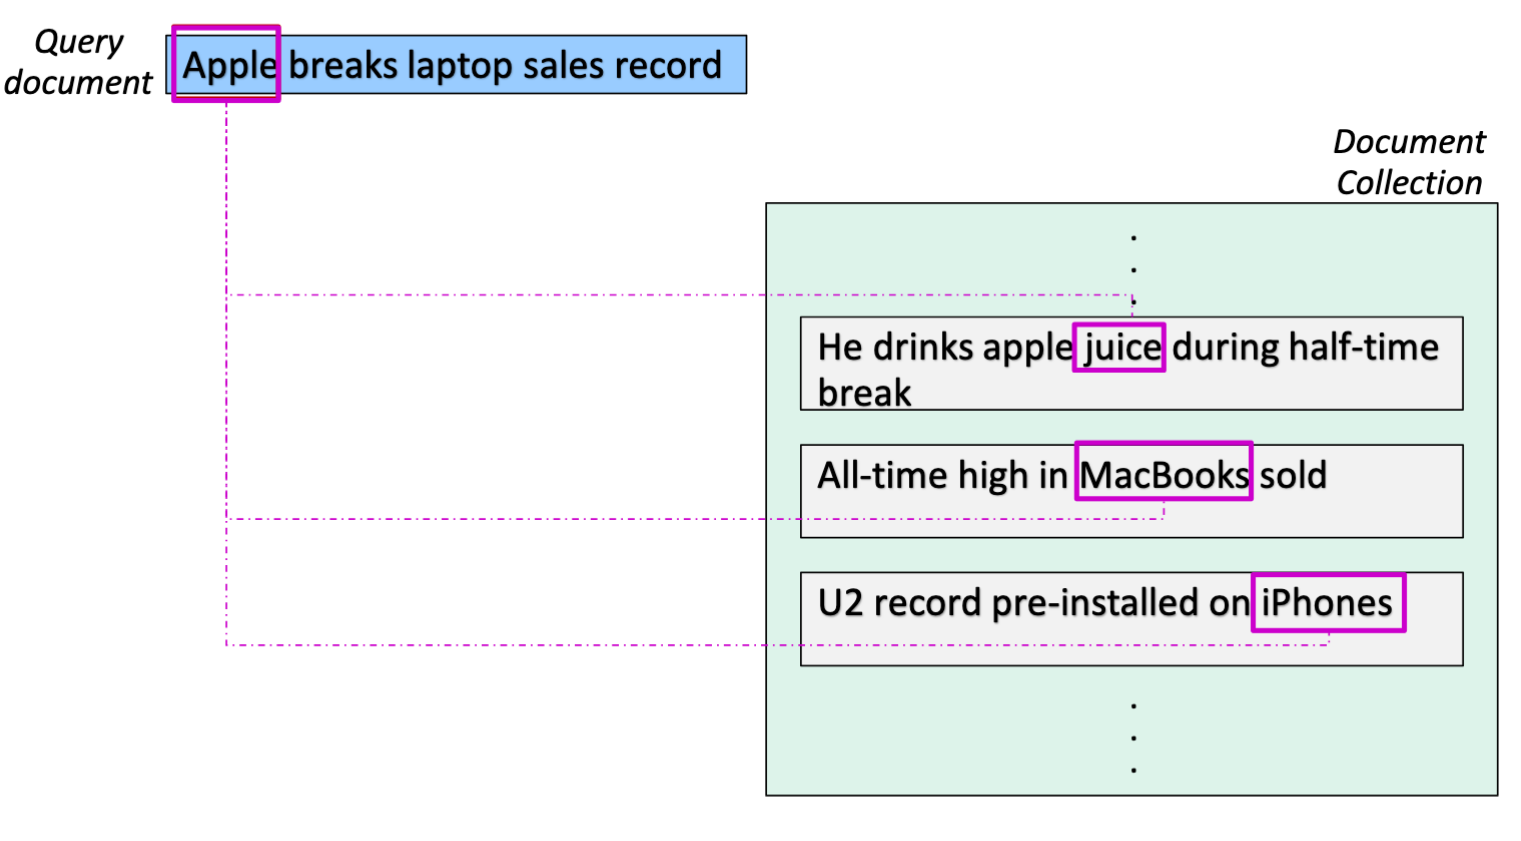
\includegraphics[width=\textwidth/2-2.08049pt]{4.png}
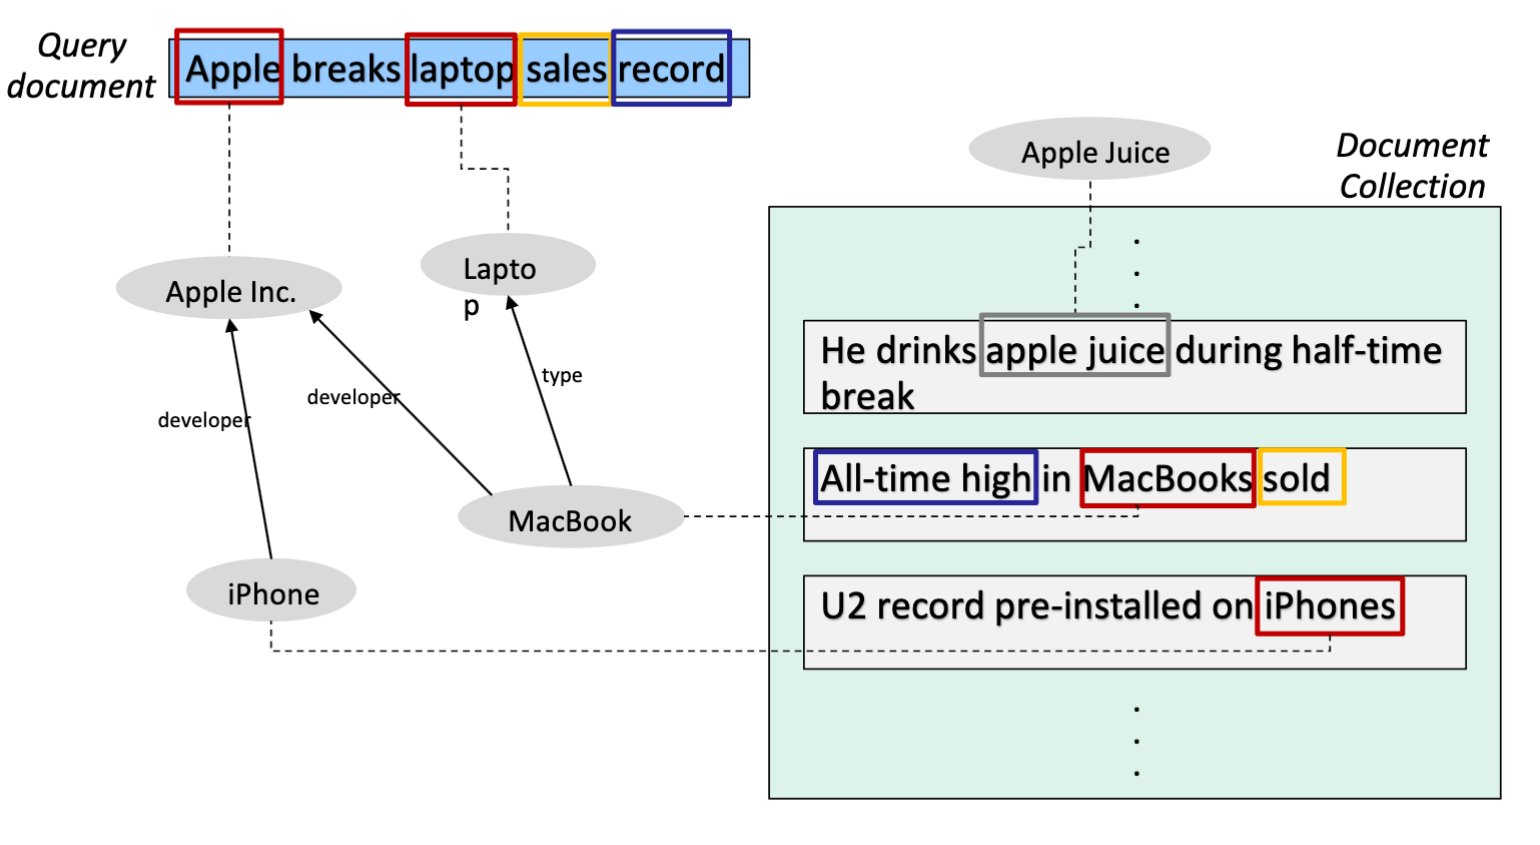
\includegraphics[width=\textwidth/2]{5.png}

Knowledge Graph Technologies:
resolve ambiguity \& exploit relational knowledge
We want apple to refer to the Apple company.
Extract noun phrases and resolve conflicts

\section{Resource Description
Framework (RDF)}

\subsection{First: Let’s get some RDF}

\begin{verbatim}
    curl --include --location --header "Accept:application/rdf+xml"
    http://dbpedia.org/resource/Yukihiro_Matsumoto
    How about Satoshi_Nakamoto?
    For human readable information, see the corresponding
    https://en.wikipedia.org/wiki/Satoshi_Nakamoto
    curl --include --location --header "Accept:application/rdf+xml"    
    http://dbpedia.org/resource/Sirius
    Who is this for?
    The web for programmers.
    Can we describe things like we do people and stars?
\end{verbatim}
 
\subsection{Each of these stores many many RDF triples.}
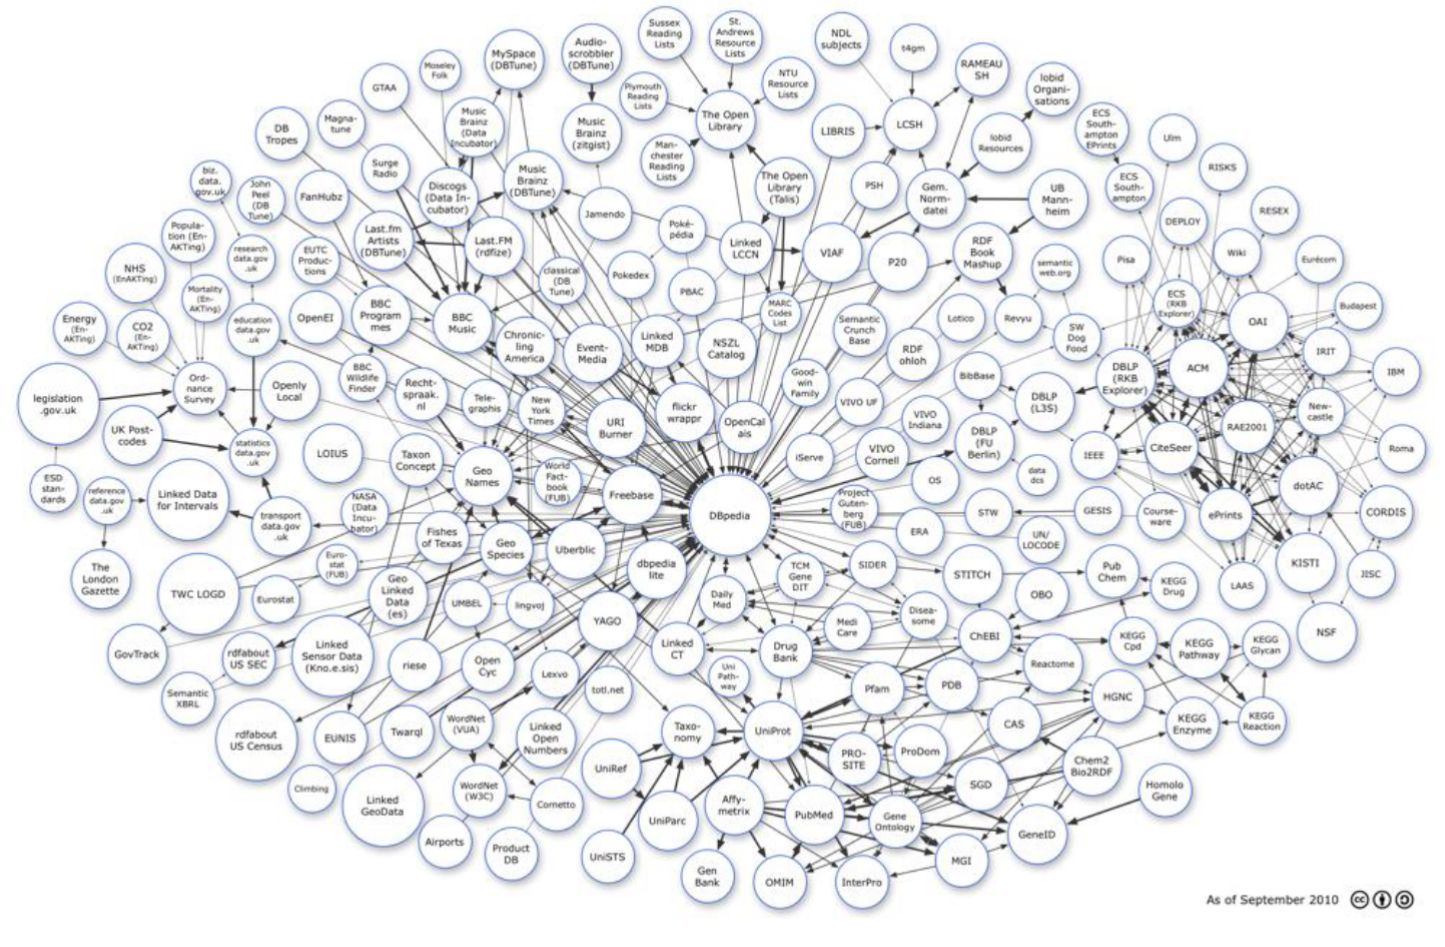
\includegraphics[width=\textwidth/2-2.08049pt]{6.png}
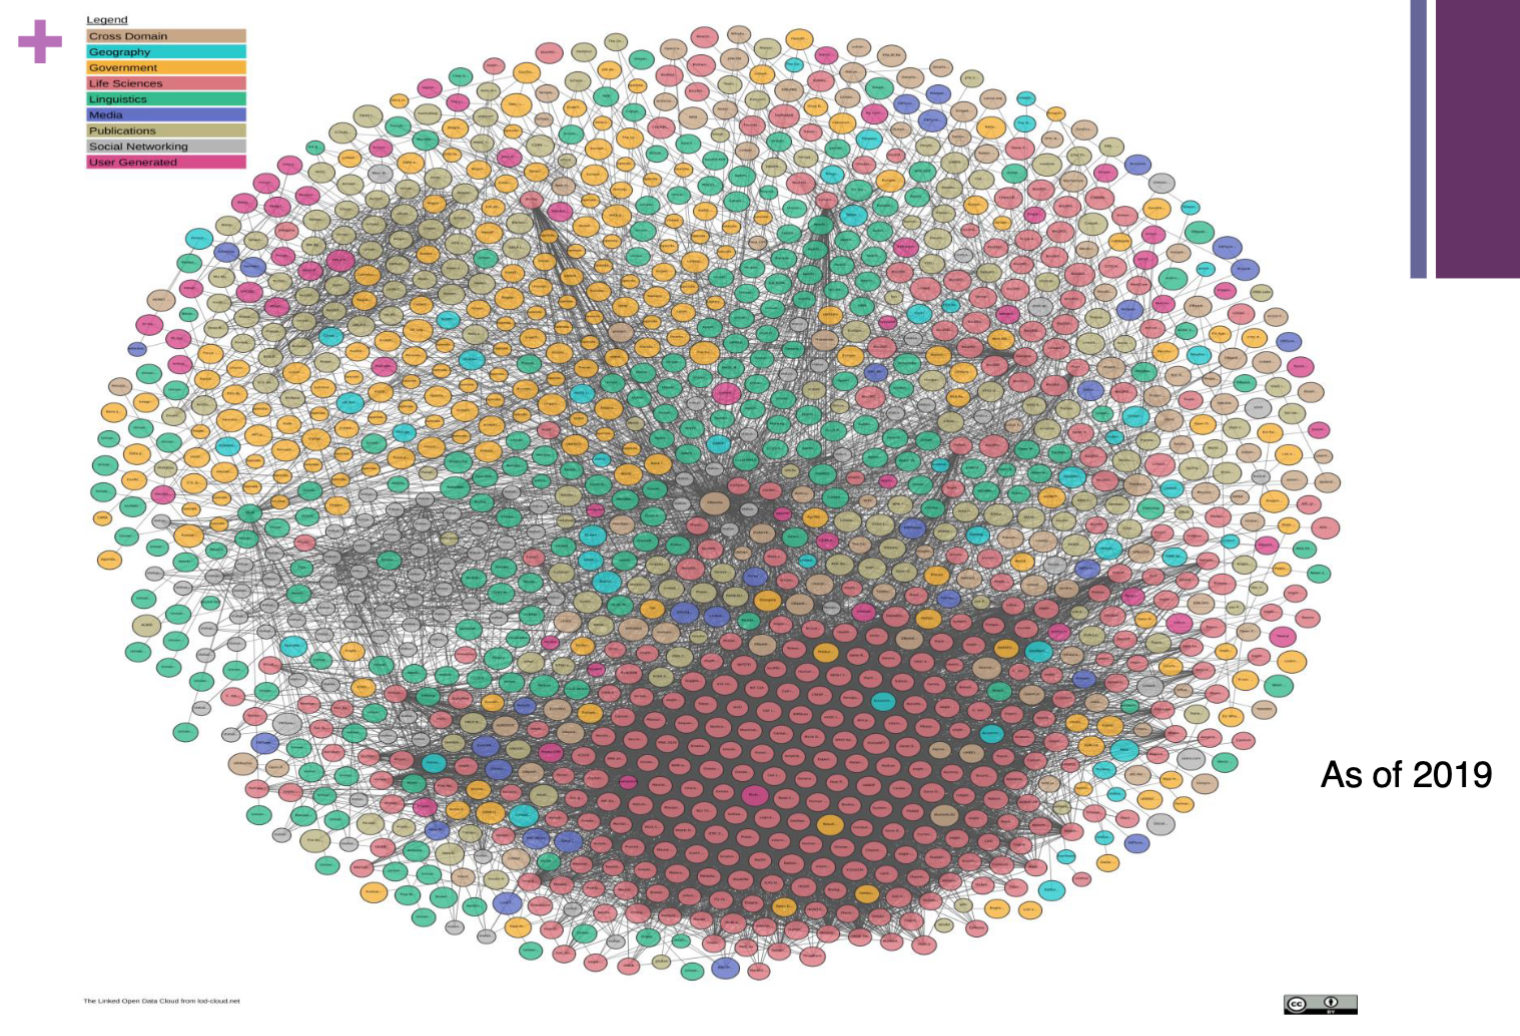
\includegraphics[width=\textwidth/2]{7.png}

\subsection{A Knowledge Graph from Triples}

most graphs are directional, right is triple format

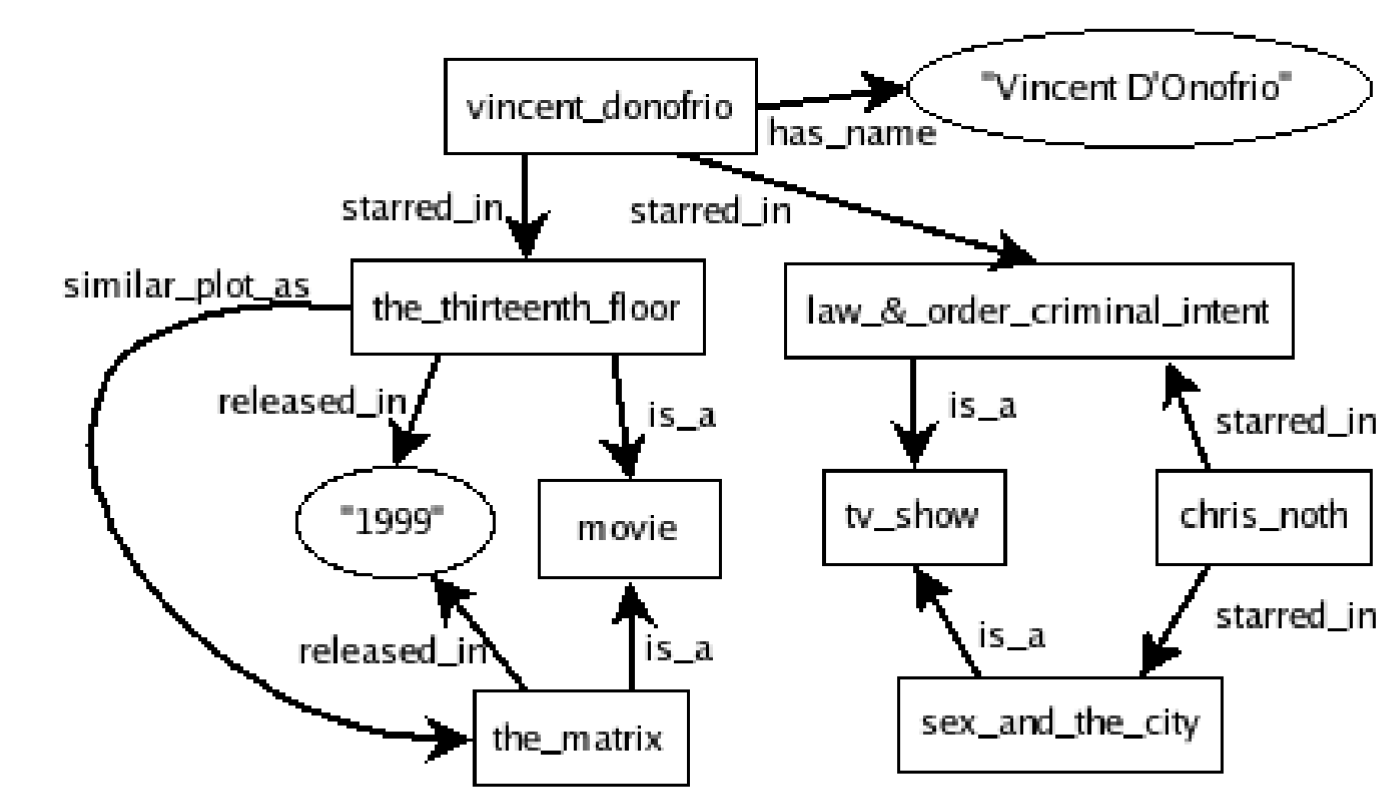
\includegraphics[width=\textwidth/2-2.08049pt]{8.png}
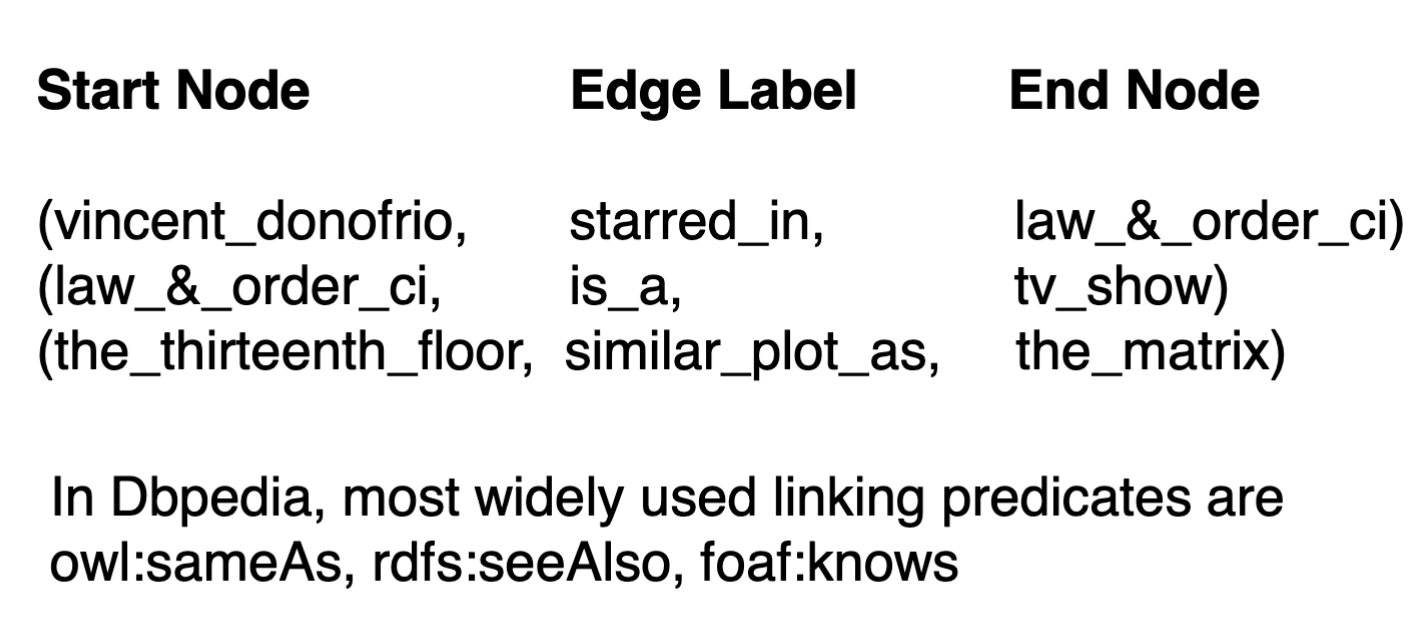
\includegraphics[width=\textwidth/2]{9.png}

\subsection{Different Formats (RDF/XML)}
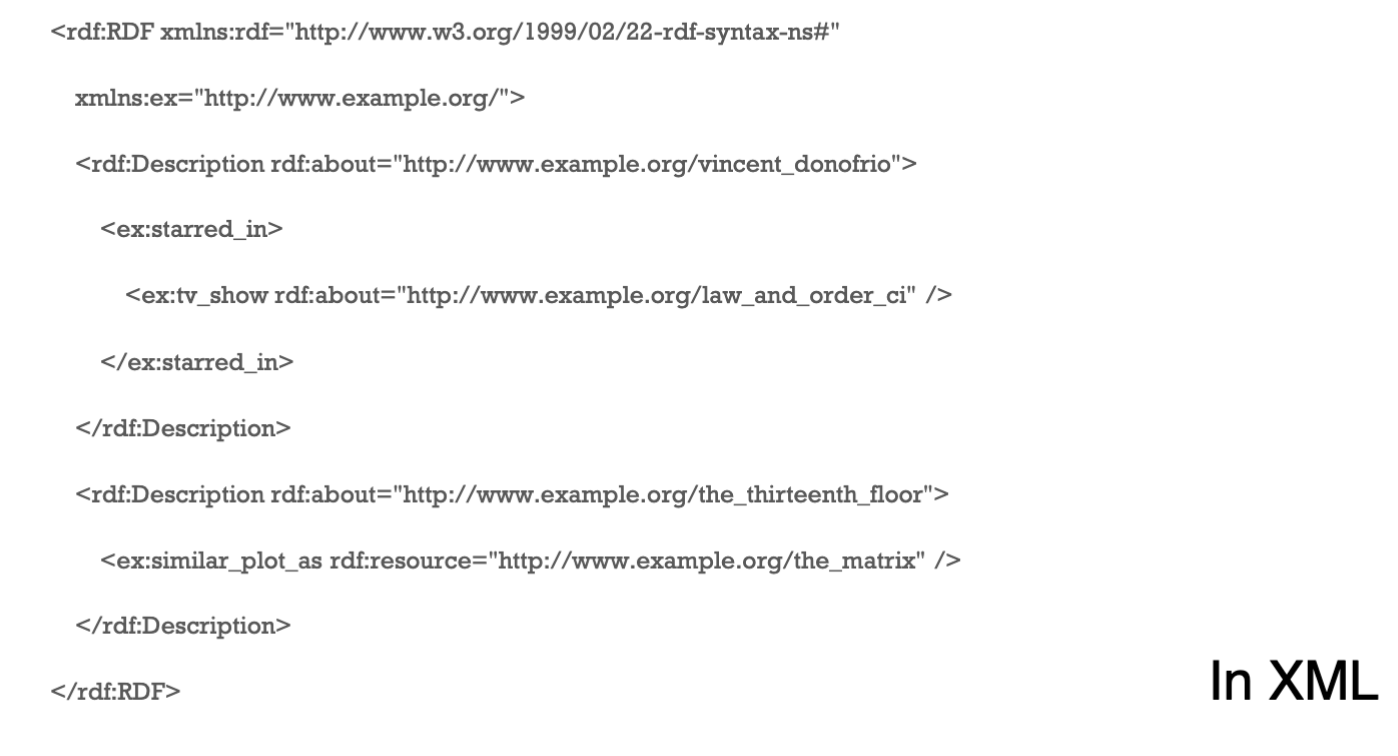
\includegraphics[width=\textwidth/2-2.08049pt]{10.png}
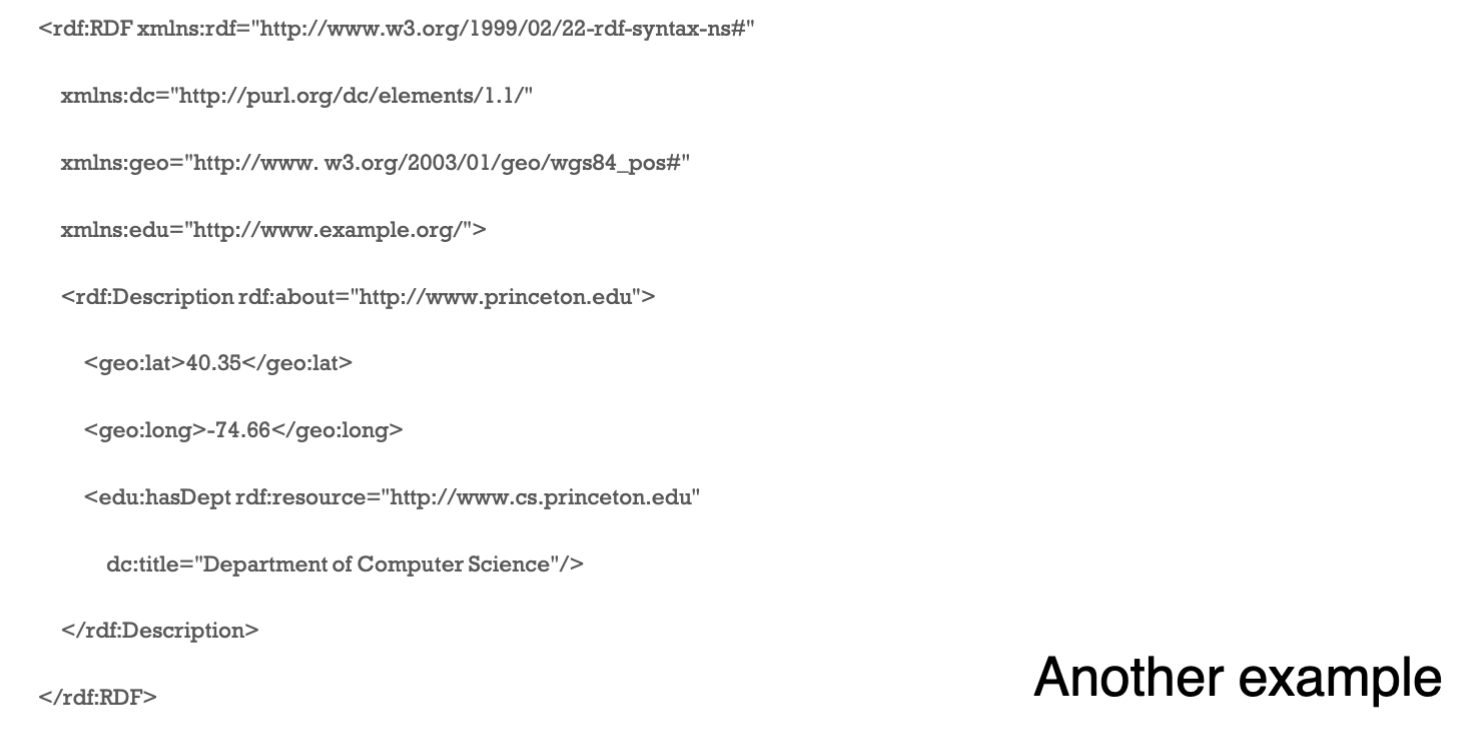
\includegraphics[width=\textwidth/2]{11.png}

\subsection{As A Table}
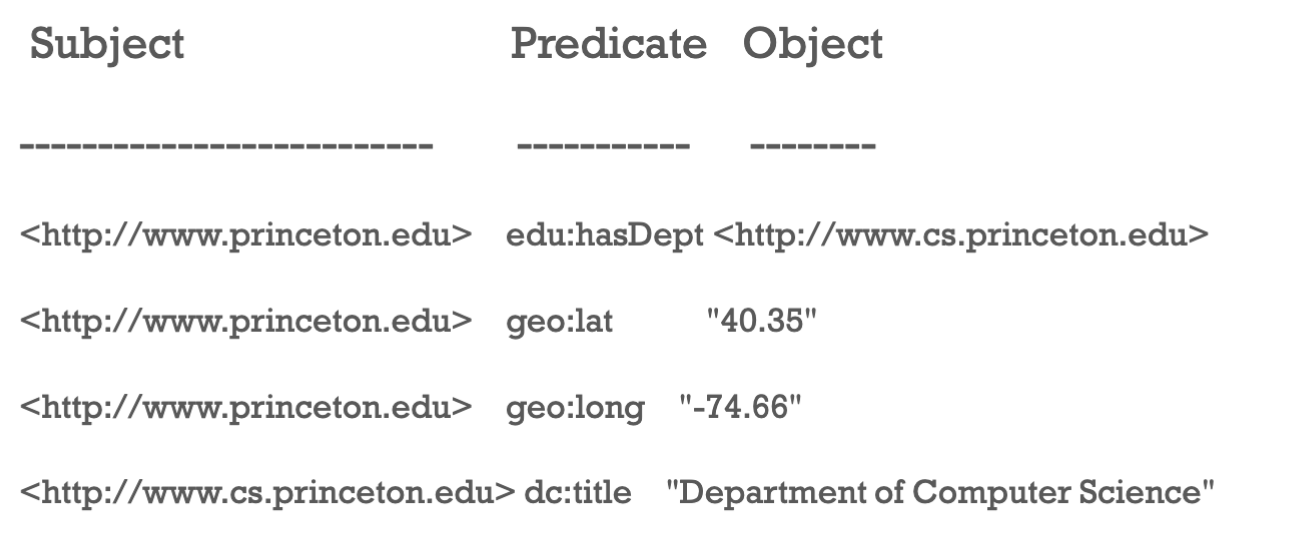
\includegraphics[width=\textwidth/2]{12.png}

\subsection{A triple may be 3 URI’s}

\begin{verbatim}
    How do we say "Billy Holiday was a songwriter" ?
    With three URI’s:
        http://dbpedia.org/resource/Billie_Holiday
        http://dbpedia-owl:occupation
        http://dbpedia.org/page/Songwriter
    In an ontology, we might learn that that all 
    Songwriters are People.
    What deduction could we make?
\end{verbatim}

\subsection{RDFa and RDF}
\begin{itemize}
    \item RDF stands on its own. Has many representations.
    \item RDFa is a lightweight version of RDF for web pages.
    \item RDFa is being used today by search engines like Google and
    sites like Best Buy.
    \item JSON-LD is being supported by W3C for WoT.
\end{itemize}

With RDFa, we can make these statements in a web page.

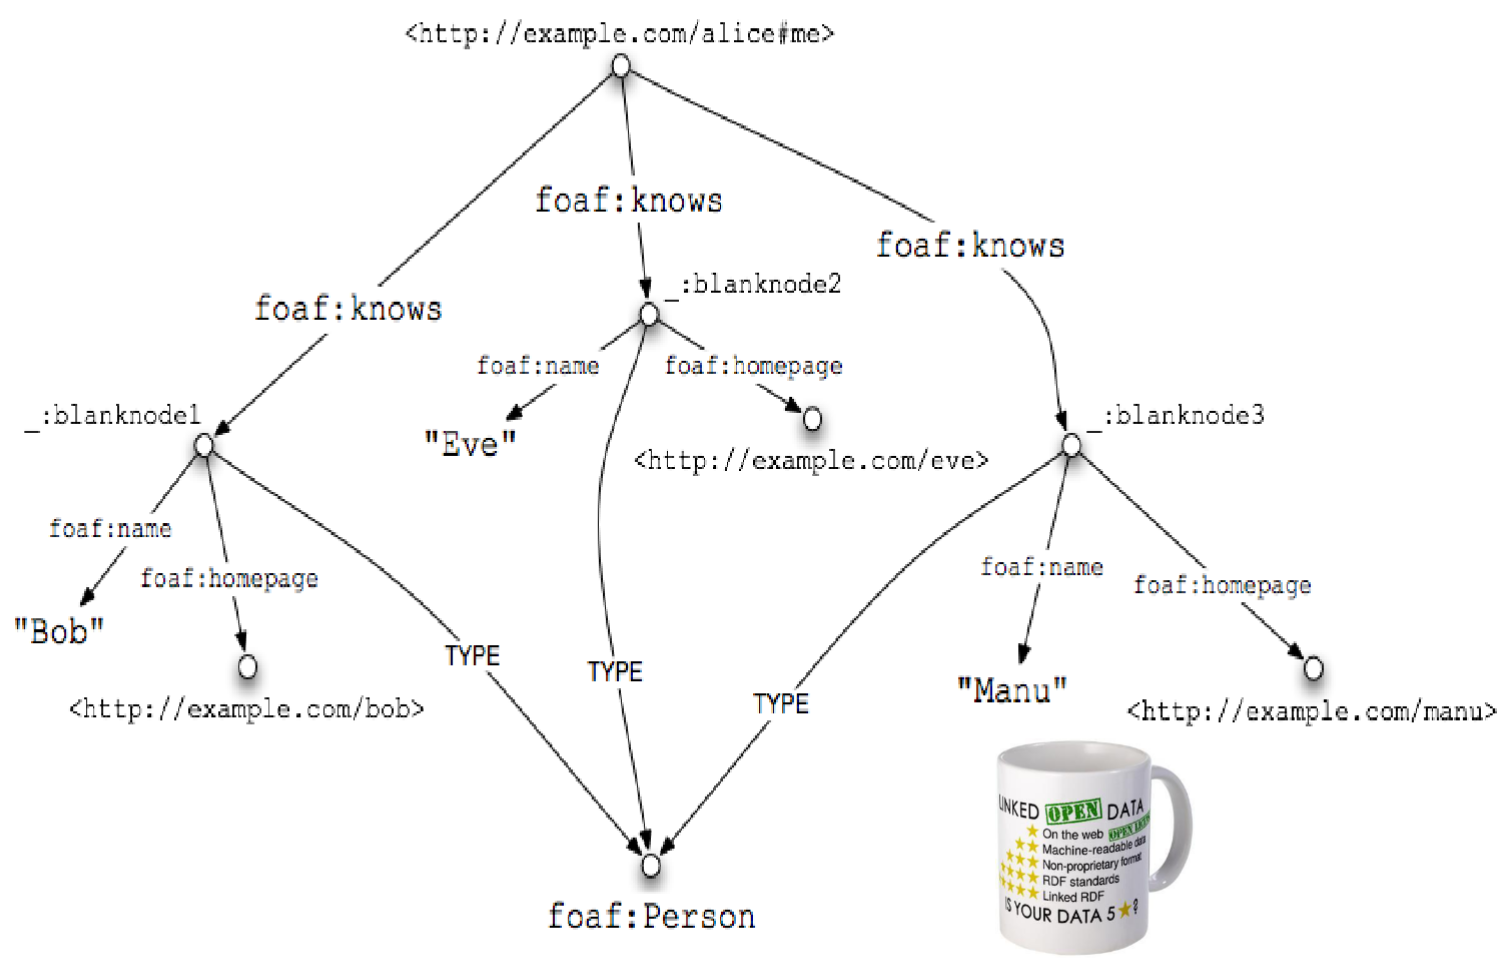
\includegraphics[width=\textwidth/2]{13.png}

\subsection{Adding RDFa}
Describing persons

\begin{verbatim}
    <div xmlns:foaf="http://xmlns.com/foaf/0.1/">
        <ul>
            <li typeof="foaf:Person">
                <a href="http://example.com/bob/">Bob</a>
            </li>
            <li typeof="foaf:Person">
                <a href="http://example.com/eve/">Eve</a>
            </li>
            <li typeof="foaf:Person">
                <a href="http://example.com/manu/">Manu</a>
            </li>
        </ul>
    </div>  
\end{verbatim}

\subsection{Add Homepages}
Describing
relationships
with rel attribute.

\begin{verbatim}
    <div xmlns:foaf="http://xmlns.com/foaf/0.1/">
        <ul>
            <li typeof="foaf:Person">
                <a rel="foaf:homepage" href="http://example.com/bob/">Bob</a>
            </li>
            <li typeof="foaf:Person">
                <a rel="foaf:homepage" href="http://example.com/eve/">Eve</a>
            </li>
            <li typeof="foaf:Person">
                <a rel="foaf:homepage" href="http://example.com/manu/">Manu</a>
            </li>
        </ul>
    </div>
\end{verbatim}

\subsection{Summary}
\begin{itemize}
    \item In MIE223, we focus on Knowledge Graphs (KGs) as a
    structured data source
    \begin{itemize}
        \item I.e., we query SPARQL and load it into Pandas table
        \begin{itemize}
            \item We’re often querying one or two sources
            \item This is probably the most common use of Knowledge Graphs
        \end{itemize}
        \item You’ll see a lot of SQL next year in Data Modelling
        \begin{itemize}
            \item For data stored internally within an organization
        \end{itemize}
    \end{itemize}
    \item But KGs are part of the Semantic Web
    \begin{itemize}
        \item The idea that structured data can be distributed around the web
        \item Updated dynamically
        \item Retrieved like you would with a Google Search
        \begin{itemize}
            \item This use of KGs has not quite taken off the way single well-
            curated sources have taken off... consider why
        \end{itemize}
    \end{itemize}
\end{itemize}

\end{document}